\chapter{Internal Resistance of a Cell}

\section{Aim}
To learn how to determine the Electromotive force (e.m.f) and internal resistance of a dry cell

\section{Background Information}
Batteries are made from materials which have resistance. This means that batteries are not only sources of potential difference (voltage), but they also possess internal resistances. If the pure voltage source is referred to as the electromotive force, E, then a battery can be represented as an emf connected in series with a resistor r. Batteries are used mainly as sources of electric power in different fields. 

The emf of a battery is essentially constant because it only depends on the chemical reaction (that converts chemical energy into electrical energy) inside the battery. Therefore, the voltage across the terminals of the battery is dependent on the current drawn by the load.

\section{Materials}
Voltmeter (0-3 V), Ammeter (0-2 A), Switch, dry cell size D, connecting wires and Rheostat (0-50 $\Omega$)

\section{Procedure}
\begin{enumerate}
\item Connect a circuit as shown in the figure.
\item Record the reading on the voltmeter when the switch $K$ is open.
\item Close the switch and adjust the rheostat so that the metal slide is furthest away from the switch.
\item Record the reading on the ammeter and voltmeter.
\item While keeping the switch closed, move the metal slide on the rheostat towards the switch to obtain five more readings of the current and voltage.
6.	Record all 6 readings of voltage and current values in tabular form.
\end{enumerate}

\begin{figure}[h!]
\centering
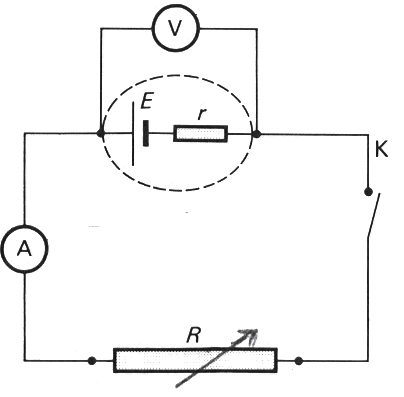
\includegraphics[width=6cm]{./img/internal-resistance-1.png}
\caption{Internal Resistance of a Cell practical setup}
\label{fig:internal-resistance-1}
\end{figure}

\section{Analysis and Interpretation}
\begin{enumerate}
\item Draw a graph of voltage against current.
\item Find the slope from the graph. What is the physical meaning of this slope?
\item What is the value of $y$-intercept of the graph and what does it represent?
\item Write the equation of the graph relating the current, $I$, and the voltage, $V$.
\end{enumerate}

\section{Conclusion}
What are the values of the electromotive force and internal resistance of your dry cell?

\section{Questions for Discussion}
\begin{enumerate}
\item How does the internal resistance affect the electromotive force of the cell when the current flows? 
\item Is the internal resistance for a new dry cell the same as for an old dry cell? Explain.
\item Why do dry cells have higher internal resistance than liquid cells (accumulators)?
\item Explain why a used dry cell will start working again when it is heated up by the sun?
\end{enumerate}

\section{Reflection and Self Assessment}
\begin{enumerate}
\item Is there anything you did not understand in this experiment? If yes, then what was it and in what ways can you increase your understanding now?
\end{enumerate}